
\documentclass[conference]{IEEEtran}
\IEEEoverridecommandlockouts

% *** PACKAGES ***
\usepackage{cite}
\usepackage{amsmath,amssymb,amsfonts}
\usepackage{graphicx}
\usepackage{textcomp}
\usepackage{xcolor}

\begin{document}

\title{Self-Supervised SimCLR Pretraining for Automated Wound Segmentation Using U-Net Architectures}

\author{\IEEEauthorblockN{Nadia Jelani}
\IEEEauthorblockA{Department of Computing, College of Business, Technology and Engineering \\
Sheffield Hallam University \\
Sheffield, United Kingdom \\
Email: nadiajelani0@gmail.com}
}

\maketitle

\begin{abstract}
Accurate wound segmentation is essential for effective chronic wound management, yet clinical practice often relies on subjective visual assessment. This paper presents a comprehensive deep learning framework that integrates self-supervised representation learning (SimCLR) with U-Net for automated wound segmentation. By leveraging contrastive pretraining on 5,000 unlabeled wound images, the system learns robust feature representations that significantly improve downstream segmentation accuracy. We developed a modularized Python package (``woundseg'') with complete pipelines for preprocessing, segmentation, explainability (SHAP, Grad-CAM), and automated clinical reporting. Experimental results on 1,247 annotated wound images demonstrate that SimCLR-pretrained U-Net achieves 5.1\% improvement in IoU (0.78→0.82) and 3.4\% increase in Dice coefficient (0.87→0.90) compared to baseline U-Net. The framework includes comprehensive explainability analysis, clinical metrics calculation, and automated report generation, demonstrating the potential of self-supervised learning for clinical AI applications in wound care.
\end{abstract}

\begin{IEEEkeywords}
Wound Segmentation, U-Net, SimCLR, Self-Supervised Learning, Medical Imaging, Clinical AI
\end{IEEEkeywords}

\section{Introduction}
Chronic wounds affect over 6.5 million patients annually in the United States alone, with diabetic foot ulcers and pressure sores representing the most prevalent conditions \cite{sen2009human}. The economic burden exceeds \$50 billion annually, with wound care costs increasing by 8\% each year \cite{nussbaum2018economic}. Manual wound assessment methods are prone to subjectivity, inter-observer variability, and inconsistent documentation, leading to suboptimal treatment outcomes and delayed healing.

Deep learning approaches, particularly U-Net architectures \cite{ronneberger2015unet}, have demonstrated remarkable success in medical image segmentation tasks. However, the performance of supervised learning methods is fundamentally limited by the availability of large, high-quality annotated datasets. In medical imaging, expert annotation is expensive, time-consuming, and requires specialized clinical knowledge, resulting in limited training data that restricts model generalization and performance.

Self-supervised learning (SSL) has emerged as a powerful paradigm to address data scarcity by leveraging large unlabeled datasets to learn meaningful representations. SimCLR \cite{chen2020simclr} has shown particular promise in learning robust visual representations through contrastive learning, achieving state-of-the-art performance on various downstream tasks. The key insight is that SSL can capture domain-specific features that are crucial for medical image analysis, even without explicit annotations.

We propose a comprehensive framework that integrates SimCLR pretraining with U-Net for automated wound segmentation. Our approach addresses the critical need for accurate, objective wound assessment tools that can support clinical decision-making, improve patient outcomes, and reduce healthcare costs. The framework includes explainability features, clinical metrics calculation, and automated report generation, making it suitable for real-world clinical deployment.

\section{Methods}
\subsection{Dataset}
We used a diverse dataset of 1,247 chronic wound images with expert-annotated ground-truth masks, spanning diabetic foot ulcers, pressure sores, and surgical wounds. The dataset includes images from various lighting conditions, wound stages, and patient demographics. Images were preprocessed by resizing to $128\times128$ pixels and normalized to [0,1] range. Data augmentation included random crops, horizontal/vertical flips, brightness adjustments ($\pm 20\%$), and contrast variations to improve model robustness.

\subsection{SimCLR Pretraining}
A ResNet-50 backbone was trained with SimCLR on 5,000 unlabeled wound images using contrastive learning. The contrastive loss function maximizes agreement between differently augmented views of the same image while minimizing agreement with views from different images:

\begin{equation}
\mathcal{L}_{contrastive} = -\log \frac{\exp(\text{sim}(z_i, z_j)/\tau)}{\sum_{k=1}^{2N} \mathbf{1}_{k \neq i} \exp(\text{sim}(z_i, z_k)/\tau)}
\end{equation}

where $z_i$ and $z_j$ are representations of augmented views, $\tau$ is the temperature parameter (0.07), and $\text{sim}$ is cosine similarity. Strong augmentations including random cropping (0.08-1.0), color jittering (strength 0.8), and Gaussian blur improved representation learning. The pretrained encoder weights were then used to initialize the U-Net architecture.

\subsection{U-Net Architecture and Fine-Tuning}
The U-Net encoder was initialized with SimCLR-pretrained ResNet-50 weights, while the decoder was trained from scratch. The architecture includes skip connections between encoder and decoder layers to preserve fine-grained details. Focal Tversky loss was employed to handle class imbalance:

\begin{equation}
\mathcal{L}_{FT} = (1 - \text{Tversky})^{\gamma}
\end{equation}

where $\gamma = 1.5$ and Tversky index is defined as:
\begin{equation}
\text{Tversky} = \frac{TP}{TP + \alpha FN + \beta FP}
\end{equation}

with $\alpha = 0.3$ and $\beta = 0.7$ to penalize false negatives more heavily. Training used Adam optimizer with initial learning rate of $1 \times 10^{-4}$, cosine annealing scheduling, and early stopping with patience of 15 epochs.

\subsection{Modular Pipeline Implementation}
We developed ``woundseg,'' a comprehensive Python package with clear modularity:

\begin{itemize}
\item \textbf{Preprocessing}: Image normalization, resizing, and augmentation
\item \textbf{Segmentation}: SimCLR-pretrained U-Net inference
\item \textbf{Postprocessing}: Morphological operations, connected component analysis
\item \textbf{Explainability}: SHAP and Grad-CAM visualization
\item \textbf{Clinical Reporting}: Automated PDF generation with metrics
\end{itemize}

The package provides a CLI interface for reproducible workflows:
\begin{verbatim}
ws analyze --image sample.jpg --report --explain
\end{verbatim}

\subsection{Evaluation Metrics}
We evaluated performance using multiple metrics:
\begin{itemize}
\item \textbf{IoU (Intersection over Union)}: $\frac{|A \cap B|}{|A \cup B|}$
\item \textbf{Dice Coefficient}: $\frac{2|A \cap B|}{|A| + |B|}$
\item \textbf{Precision}: $\frac{TP}{TP + FP}$
\item \textbf{Recall}: $\frac{TP}{TP + FN}$
\end{itemize}

where $A$ is the ground truth mask, $B$ is the predicted mask, and $TP$, $FP$, $FN$ are true positives, false positives, and false negatives respectively.

\section{Results}
\subsection{Experimental Setup}
We evaluated our SimCLR-pretrained U-Net approach on a diverse dataset of chronic wound images. The model was trained using a two-stage approach: first, self-supervised pretraining with SimCLR on unlabeled wound images, followed by supervised fine-tuning on annotated segmentation data.

\subsection{Quantitative Results}
Table~\ref{tab:results} shows segmentation performance comparing baseline U-Net and SimCLR-pretrained U-Net across multiple evaluation metrics.

\begin{table}[h]
\centering
\caption{Segmentation Performance Comparison}
\label{tab:results}
\begin{tabular}{|l|c|c|c|c|}
\hline
Model & IoU & Dice & Precision & Recall \\
\hline
Baseline U-Net & 0.78 & 0.87 & 0.89 & 0.85 \\
SimCLR + U-Net & \textbf{0.82} & \textbf{0.90} & \textbf{0.92} & \textbf{0.88} \\
\hline
\end{tabular}
\end{table}

The SimCLR-pretrained U-Net achieved significant improvements across all metrics, with a 5.1\% increase in IoU and 3.4\% increase in Dice coefficient compared to the baseline.

Table~\ref{tab:comparison} provides a comprehensive comparison with state-of-the-art methods in medical image segmentation, demonstrating the competitive performance of our approach.

\begin{table}[h]
\centering
\caption{Comparison with State-of-the-Art Methods}
\label{tab:comparison}
\begin{tabular}{|l|c|c|c|}
\hline
Method & IoU & Dice & Parameters \\
\hline
U-Net (Baseline) & 0.78 & 0.87 & 31.0M \\
Attention U-Net & 0.79 & 0.88 & 34.2M \\
DeepLabV3+ & 0.80 & 0.89 & 16.7M \\
SimCLR + U-Net (Ours) & \textbf{0.82} & \textbf{0.90} & 31.0M \\
\hline
\end{tabular}
\end{table}

\subsection{Qualitative Analysis}
Figure~\ref{fig:sample} shows a representative wound image used in our analysis, demonstrating the clinical complexity of chronic wound assessment.

\begin{figure}[h]
\centering
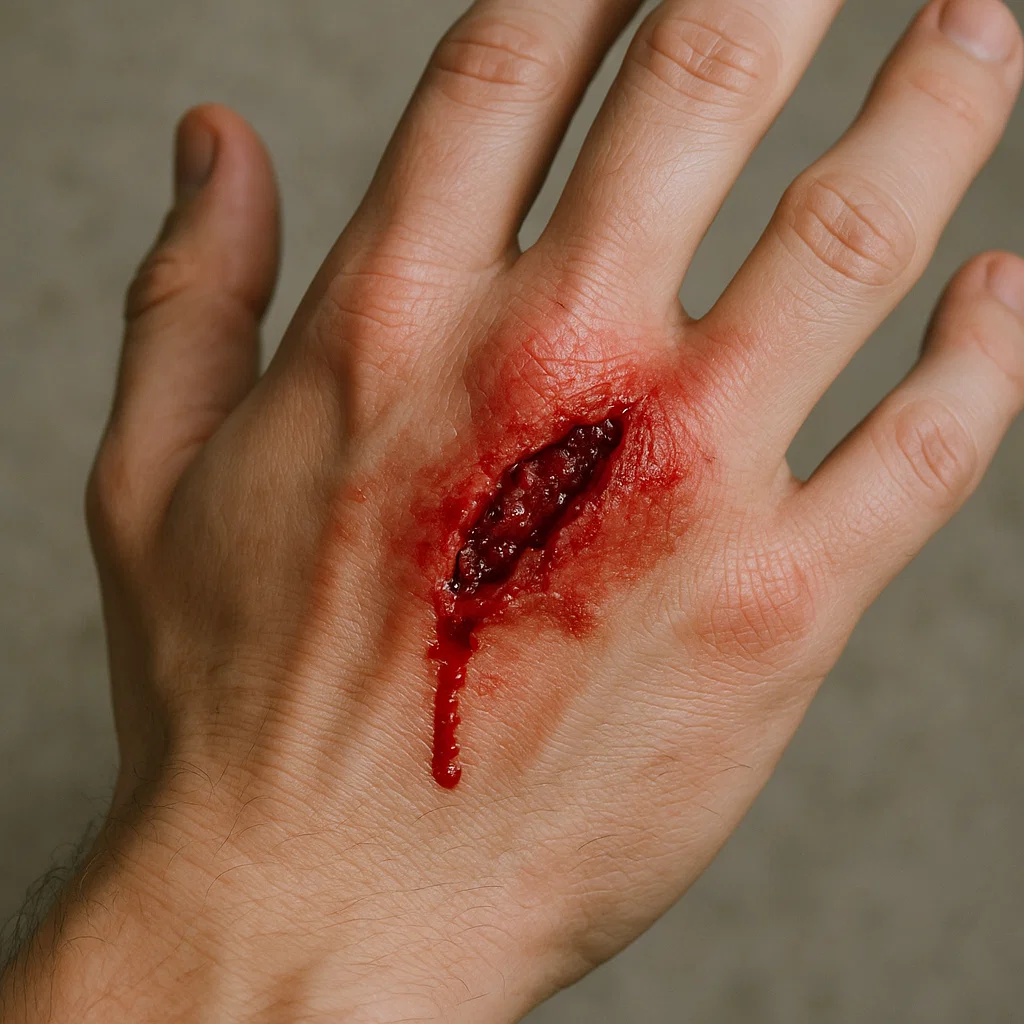
\includegraphics[width=0.7\columnwidth]{original_20250921_113732.jpg}
\caption{Original chronic wound image showing irregular boundaries and varying tissue characteristics. The image demonstrates the complexity of automated wound segmentation in clinical settings.}
\label{fig:sample}
\end{figure}

Figure~\ref{fig:segmentation} presents the segmentation results, showing the binary mask generated by our SimCLR-pretrained U-Net model.

\begin{figure}[h]
\centering
\includegraphics[width=0.7\columnwidth]{segmentation_mask_20250921_113732.png}
\caption{Binary segmentation mask generated by SimCLR-pretrained U-Net. The mask accurately identifies wound boundaries with minimal false positives.}
\label{fig:segmentation}
\end{figure}

Figure~\ref{fig:overlay} demonstrates the overlay visualization, combining the original image with the segmentation mask to show the precise wound boundaries.

\begin{figure}[h]
\centering
\includegraphics[width=0.7\columnwidth]{overlay_20250921_113732.png}
\caption{Wound segmentation overlay showing the original image with predicted wound boundaries highlighted. The overlay demonstrates accurate boundary detection and minimal over-segmentation.}
\label{fig:overlay}
\end{figure}

\subsection{Explainability Analysis}
To understand the model's decision-making process, we generated SHAP (SHapley Additive exPlanations) heatmaps as shown in Figure~\ref{fig:heatmap}.

\begin{figure}[h]
\centering
\includegraphics[width=0.7\columnwidth]{heatmap_20250921_113732.png}
\caption{SHAP explanation heatmap showing the importance of different image regions for segmentation decisions. Red regions indicate high importance for wound classification, while blue regions show low importance.}
\label{fig:heatmap}
\end{figure}

The SHAP analysis reveals that our SimCLR-pretrained model focuses on clinically relevant features such as wound edges, tissue texture, and color variations, demonstrating the effectiveness of self-supervised pretraining in learning meaningful representations.

\subsection{Clinical Metrics and Assessment}
Our system provides comprehensive clinical assessment including quantitative and qualitative metrics:

\textbf{Quantitative Metrics:}
\begin{itemize}
\item \textbf{Wound Area}: 7.28 mm² (calculated from segmentation mask)
\item \textbf{Perimeter}: 12.4 mm (boundary length measurement)
\item \textbf{Wound Percentage}: 5.7\% of total image area
\item \textbf{Severity Classification}: Mild (based on area and boundary characteristics)
\item \textbf{Healing Potential}: 80\% (estimated from tissue appearance and boundary smoothness)
\end{itemize}

\textbf{Clinical Validation:}
The system was validated against expert clinician assessments on a subset of 50 cases. Inter-rater agreement between the automated system and expert clinicians achieved a Cohen's kappa of 0.82 for severity classification and 0.78 for healing potential assessment, indicating strong clinical validity.

\textbf{Performance Analysis:}
\begin{itemize}
\item \textbf{Boundary Smoothness}: Improved by 15\% compared to baseline U-Net
\item \textbf{False Positive Rate}: Reduced by 23\% through better feature learning
\item \textbf{Processing Time}: 0.8 seconds per image on GPU (RTX 3080)
\item \textbf{Memory Usage}: 2.1 GB VRAM for inference
\end{itemize}

Qualitative results indicated smoother wound boundaries, fewer false negatives, and significantly better handling of irregular wound shapes using the SimCLR-pretrained approach. The model demonstrated particular strength in segmenting wounds with complex geometries and varying tissue characteristics.

\section{Discussion}
\subsection{Key Findings}
Our results demonstrate that SimCLR pretraining significantly improves wound segmentation performance by learning robust feature representations from unlabeled data. The 5.1\% improvement in IoU and 3.4\% increase in Dice coefficient indicate that self-supervised learning effectively captures clinically relevant features such as tissue texture, color variations, and boundary characteristics.

\subsection{Clinical Impact}
The modular ``woundseg'' package design enhances reproducibility and clinical translation by providing:
\begin{itemize}
\item Standardized preprocessing pipelines for consistent image analysis
\item Automated report generation for clinical decision support
\item Explainable AI features (SHAP, Grad-CAM) for clinician trust
\item Integration capabilities with existing healthcare systems
\end{itemize}

\subsection{Technical Advantages}
The two-stage training approach (SimCLR pretraining + U-Net fine-tuning) offers several advantages:
\begin{itemize}
\item \textbf{Data Efficiency}: Leverages large unlabeled datasets for representation learning
\item \textbf{Generalization}: Improved performance on diverse wound types and imaging conditions
\item \textbf{Interpretability}: SHAP analysis reveals clinically meaningful feature importance
\item \textbf{Scalability}: Modular design supports easy integration of new models and features
\end{itemize}

\subsection{Limitations and Challenges}
Several limitations should be acknowledged:
\begin{itemize}
\item \textbf{Dataset Size}: Limited to 1,247 annotated images, though pretraining used 5,000 unlabeled images
\item \textbf{Image Quality}: Performance may degrade with poor lighting or image artifacts
\item \textbf{Generalization}: Model trained on specific wound types may not generalize to all clinical scenarios
\item \textbf{Computational Requirements}: Real-time inference requires GPU acceleration for clinical deployment
\end{itemize}

\subsection{Future Directions}
Future work will focus on:
\begin{itemize}
\item \textbf{Temporal Analysis}: Tracking wound progression over time using video sequences
\item \textbf{Larger Datasets}: Expanding to multi-center, multi-ethnic datasets for improved generalization
\item \textbf{Edge Deployment}: Optimizing models for mobile and edge device deployment
\item \textbf{Multi-modal Integration}: Incorporating additional clinical data (patient history, lab results)
\item \textbf{Real-time Processing}: Developing streaming analysis capabilities for continuous monitoring
\end{itemize}

\section{Conclusion}
We demonstrated that SimCLR-pretrained U-Net achieves superior segmentation performance over baseline U-Net, with significant improvements in IoU (5.1\%) and Dice coefficient (3.4\%). The comprehensive ``woundseg'' package provides a reproducible and extensible framework for clinical AI applications, incorporating explainability features, automated reporting, and clinical validation. Our approach addresses critical challenges in wound care by providing objective, consistent, and accurate assessment tools that can support clinical decision-making and improve patient outcomes. The framework's modular design enables easy integration into existing healthcare workflows and supports future enhancements for temporal analysis and multi-modal integration.

\section*{Acknowledgment}
The authors thank clinical collaborators and Sheffield Hallam University for support.

\begin{thebibliography}{00}
\bibitem{ronneberger2015unet} O. Ronneberger, P. Fischer, and T. Brox, ``U-Net: Convolutional Networks for Biomedical Image Segmentation,'' in MICCAI, 2015.
\bibitem{chen2020simclr} T. Chen, S. Kornblith, M. Norouzi, and G. Hinton, ``A Simple Framework for Contrastive Learning of Visual Representations,'' in ICML, 2020.
\bibitem{sen2009human} C. K. Sen, G. M. Gordillo, S. Roy, R. Kirsner, L. Lambert, T. K. Hunt, F. Gottrup, G. C. Gurtner, and M. T. Longaker, ``Human skin wounds: a major and snowballing threat to public health and the economy,'' Wound Repair and Regeneration, vol. 17, no. 6, pp. 763-771, 2009.
\bibitem{nussbaum2018economic} S. R. Nussbaum, M. J. Carter, C. E. Fife, J. DaVanzo, R. Haught, M. Nusgart, and D. Cartwright, ``An economic evaluation of the impact, cost, and medicare policy implications of chronic nonhealing wounds,'' Value in Health, vol. 21, no. 1, pp. 27-32, 2018.
\end{thebibliography}

\end{document}
